%!TEX TS-program = pdflatexmk
%!TEX root = ../handbook.tex

% Copyright 2018 Martin Scheidt (ISC license)
% Permission to use, copy, modify, and/or distribute this file for any purpose with or without fee is hereby granted, provided that the above copyright notice and this permission notice appear in all copies.

\begin{tabular}{rcc}
  \toprule
  & 
    \IfLanguage{english}{halt}
    \IfLanguage{ngerman}{Halt}
  &
    \IfLanguage{english}{proceed}
    \IfLanguage{ngerman}{Fahrt}
  \\
  \hline
    \IfLanguage{english}{main signal}
    \IfLanguage{ngerman}{Hauptsignal}
  &
  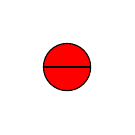
\begin{tikzpicture}[anchor=base,baseline=-3]
    \draw [fill=red] (0,0) circle (0.3);
    \draw (-0.3,0) -- (0.3,0);
    \path (-0.5,-0.5) rectangle ++(1,1); % background rectangle to unify every cell containing a symbol
  \end{tikzpicture} &
  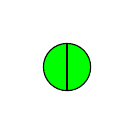
\begin{tikzpicture}[anchor=base,baseline=-3]
    \draw [fill=green] (0,0) circle (0.3);
    \draw (0,-0.3) -- (0,0.3);
    \path (-0.5,-0.5) rectangle ++(1,1); % background rectangle to unify every cell containing a symbol
  \end{tikzpicture}
  \\
    \IfLanguage{english}{distant signal}
    \IfLanguage{ngerman}{Vorsignal}
  &
  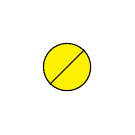
\begin{tikzpicture}[anchor=base,baseline=-3]
    \draw [fill=yellow] (0,0) circle (0.3);
    \draw (-0.22,-0.22) -- ++(0.44,0.44);
    \path (-0.5,-0.5) rectangle ++(1,1); % background rectangle to unify every cell containing a symbol
  \end{tikzpicture} &
  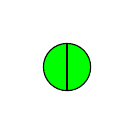
\begin{tikzpicture}[anchor=base,baseline=-3]
    \draw [fill=green] (0,0) circle (0.3);
    \draw (0,-0.3) -- (0,0.3);
    \path (-0.5,-0.5) rectangle ++(1,1); % background rectangle to unify every cell containing a symbol
  \end{tikzpicture} \\
  \bottomrule
\end{tabular}
